\chapter{E2EE \& TOR}

\section{End to End encryption}

The overall goal of Information Security is preserving the integrity and/or confidentiality of the data from its sending point to the receiving point in a network. Information Security must also provide for the receiver to be certain that the sender is actually the entity that the information was received from (authenticity). In the context of networks, these properties can be achieved by using the notion of end-to-end encryption.
Not only the communication stays encrypted during transport but also that the provider of the communication service is not able to decrypt the communications either by having access to the private key or by having the capability to undetectably inject an adversarial public key as part of a man-in-the-middle attack.
Encryption-In-Transit is different from End-to-End encryption because in the Encryption-In-Transit the communication is encrypted only from client to server, and vice versa, but the server can decrypt the communication. In the case of End-To-End encryption, the communication stays encrypted even when transiting on the server.

Weakening/suppression of E2EE is dangerous for democracy and can have a negative impact on our fundamental rights and freedom.

\subsection{Security of E2EE}

It is still vulnerable to Man-in-the-Middle attack, if the attacker can interfere with the key exchange protocol. To prevent this, Certificates (assuming a public key infrastructure is available), Web-of-trust, Fingerprints (short sequence of bytes used to identify longer public keys) are used.

E2EE does not solve the problem that users' computer can still be hacked and private keys can be stolen that way.

E2EE should guarantee the following desired properties:
\begin{itemize}
	\item Authentication: when information is received from a source, authentication means that the source is indeed as alleged in the information. The information was not altered along the way (integrity)
	\item Confidentiality: the information is safe from being eavesdropped on during its transit from the sending point to the receiving point
	\item Choosing the best security parameters and key management. The choice refers to the fact that, in general, the two endpoints of a communication link may possess different computational capabilities and, also, in general, may not have access to exactly the same set of security algorithms. Key management refers to providing solutions to the sort of practical problems that arise when users possess multiple public/private key pairs
\end{itemize}

\section{PGP}

\subsection{Authentication}
Sender authentication consists of the sender attaching its digital signature to the email and the receiver verifying the signature using public-key cryptography \ref{fig:gpg-authentication}.

\begin{figure}
	\centering
	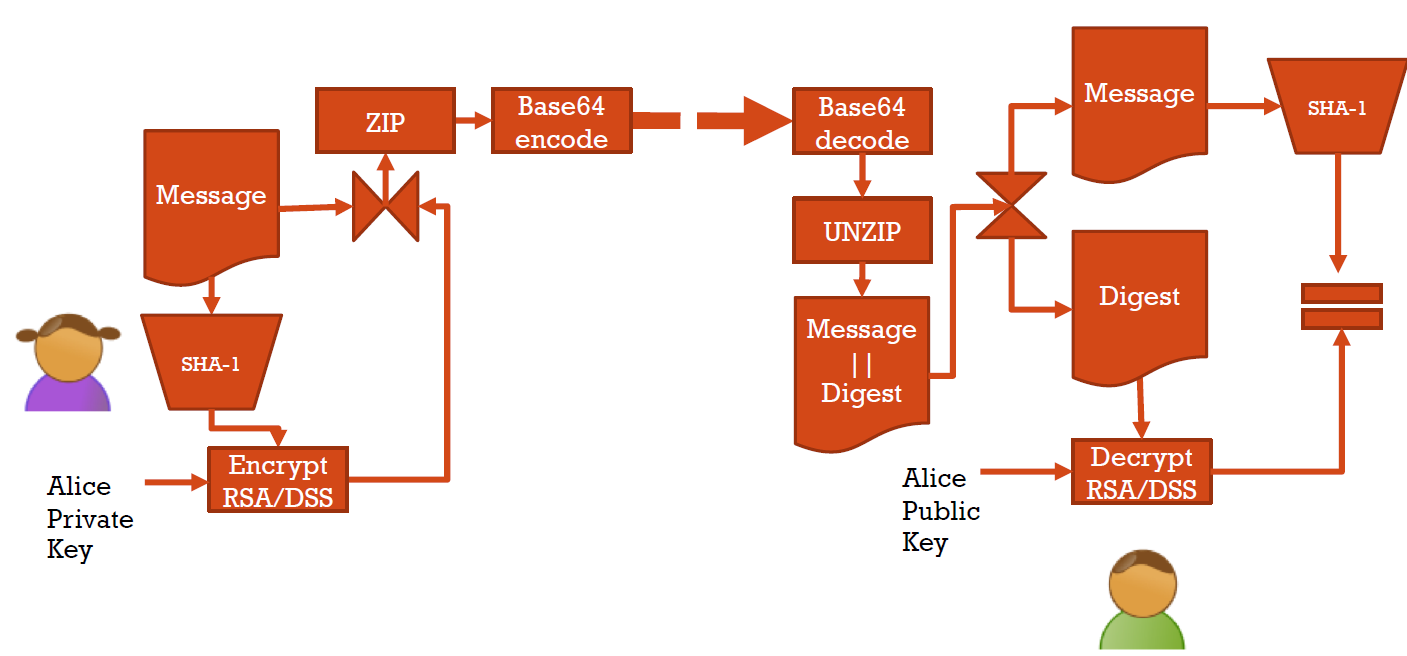
\includegraphics[width=0.7\linewidth]{Images/Chapter7/pgp-authentication}
	\caption{PGP Mode Authentication Only}
	\label{fig:gpg-authentication}
\end{figure}

\subsection{Confidentiality}

PGP uses symmetric-key encryption for confidentiality. The CAST-128,IDEA,3DES block ciphers are supported \ref{fig:pgp-confidentiality}.

\begin{figure}
	\centering
	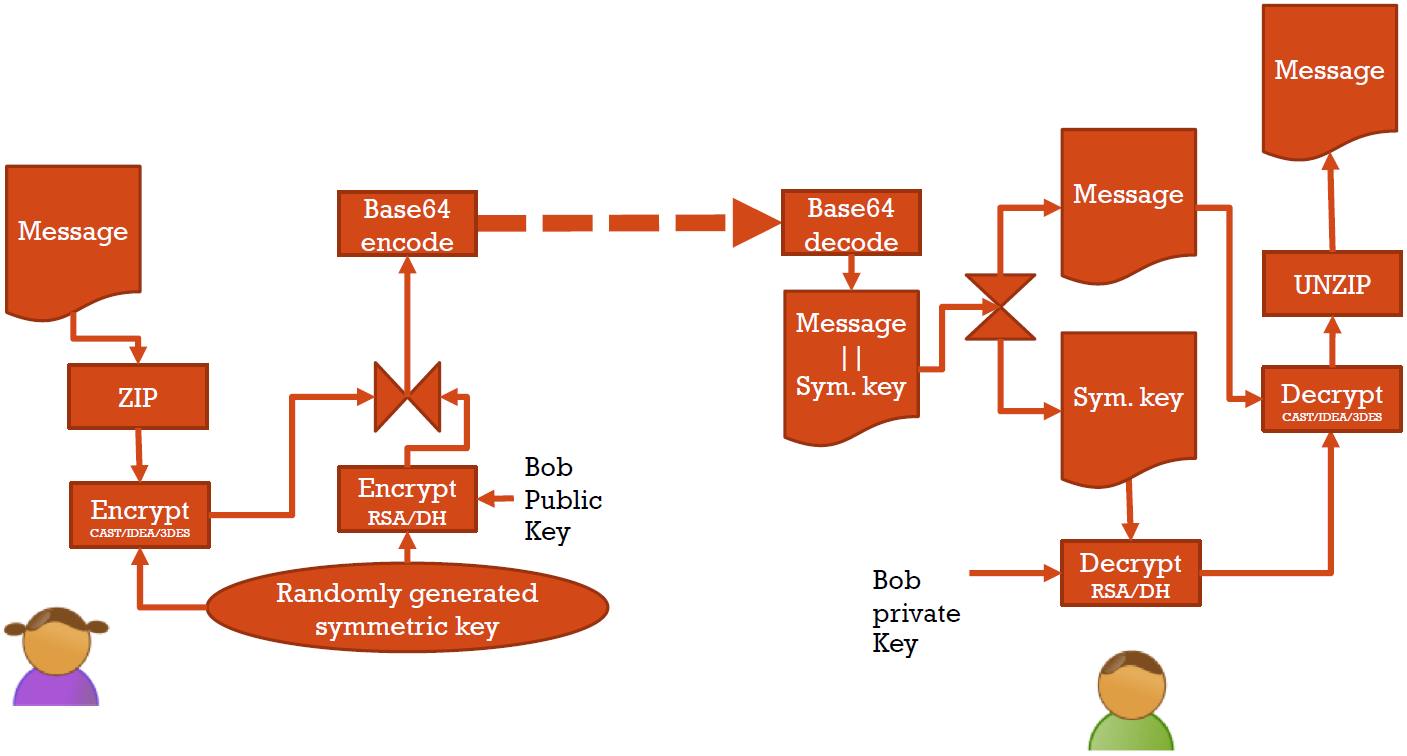
\includegraphics[width=0.7\linewidth]{Images/Chapter7/pgp-confidentiality}
	\caption{PGP Mode Confidentiality Only}
	\label{fig:pgp-confidentiality}
\end{figure}

The block ciphers are used in the Cipher Feedback Mode (CFB) \ref{sec:CipherFeedback}. The encryption key (session key) is generated for each email message separately. The session key is encrypted using RSA with the receiver's public key. Alternatively, the session key can also be established using the El Gamal algorithm. 

The message sent over the network is the email message after it is encrypted first with the session key and then with the receiver's public key. If confidentiality and sender-authentication are needed simultaneously, a digital signature for the message is generated using the hash code of the message plaintext and appended to the email message before it is encrypted with the session key.

\section{PGP Services}
\subsection{Compression}

By default, PGP compresses the email message after appending the signature but before encryption. This makes long-term storage of messages and their signatures more efficient. This also decouples the encryption algorithm from the message verification procedures. Compression is carried out with the ZIP algorithm.

\subsection{Compatibility}

Since encryption, even when it is limited to the signature, results in arbitrary binary strings. Since network message transmission is character oriented, one must represent binary data with ASCII strings. PGP uses Base64 encoding for this purpose. Base64 is a widely used encoding method to guarantee interoperability across different platforms and exchange binary data over networks.

\subsection{Segmentation}

For long email messages (generally messages containing attachments), many
email systems place restrictions on how much of the message will be transmitted as a unit. For example, some email systems segment long email messages into 50,000 byte segments and transmit each segment separately. PGP has built-in facilities for such segmentation and re-assembly.

\subsection{Message format}

The PGP message format \ref{fig:pgp-message-format}.

\begin{figure}
	\centering
	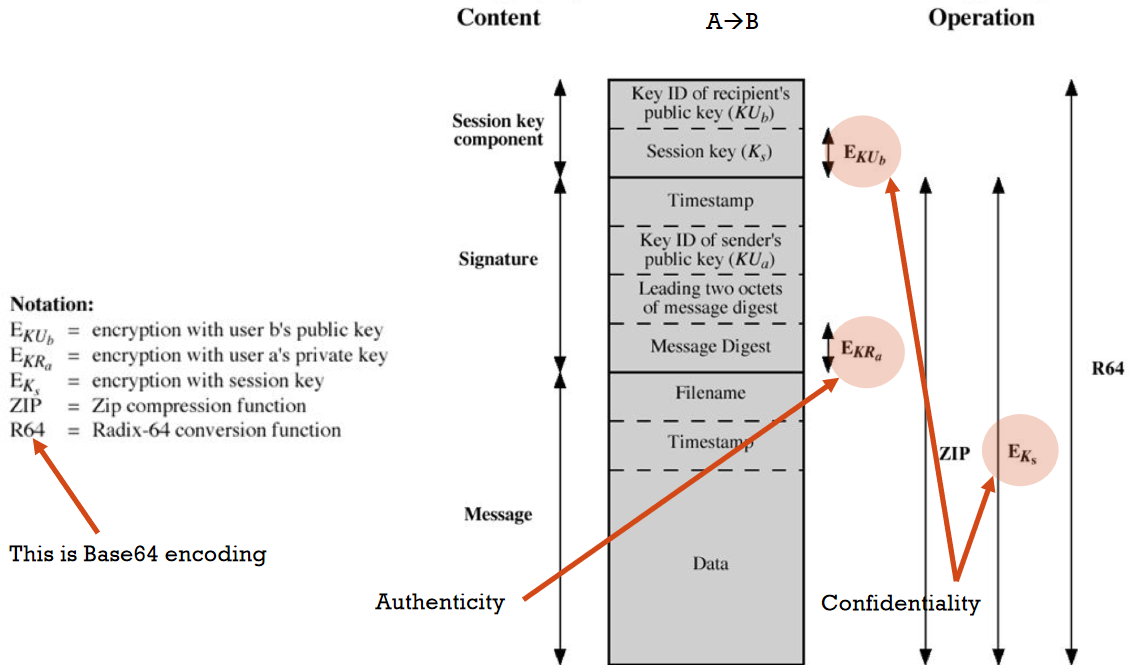
\includegraphics[width=0.7\linewidth]{Images/Chapter7/pgp-message-format}
	\caption{PGP message format}
	\label{fig:pgp-message-format}
\end{figure}



\section{Web of Trust}

Public key encryption is central to PGP as it is used for both authentication and for confidentiality. A sender uses its private key for placing its digital signature on the outgoing message. A sender uses the receiver's public key for encrypting the symmetric key used for
content encryption for ensuring confidentiality. People are likely to have multiple public and private keys for a number of different practical reasons. For example, an individual may wish to drop an old public key, but, to allow for a smooth transition, may decide to make available both the old and the new public keys for a while. PGP must allow for the possibility that the receiver of a message may have stored multiple public keys for a given sender. 
There are two questions: PGP uses one of the public keys made available by the recipient, how does the recipient know which public key it is? Next, the sender uses one of the multiple private keys that at its disposal for signing the message, how does the recipient know which of the corresponding public keys to use?  Both of these problems can be solved by the sender also including the public key used, this is indeed a waste in space because RSA public keys can be very large (and getting larger and larger for security as time went by).

PGP solves these problems by using the notion of a relatively short key identifier (called key ID) and requiring that every PGP agent maintain its own list of paired private/public keys in what is called as a Private Key Ring a list of the public keys for all its email correspondents in what is called as the Public Key Ring. Key IDs are included in messages so that the recipient of the message knows which public key to use by using its Public Key Ring. A Private Key Ring contains the public/private key pairs for a user.

The private key ring contains:
\begin{itemize}
	\item Timestamp: date/time when key pair generated
	\item Key ID: least significant 64 bits of public key
	\item Public key: public-key portion of the pair
	\item Private key: private key portion of the pair this field is encrypted
\end{itemize}

The public key ring contains: Timestamp, Key ID, Public Key, and User ID have the same meaning as in the private key ring. The remaining fields are used for handling trust Owner Trust, Key Legitimacy, Signature(s), and Signature Trusts are used to assess how much trust to place in the public keys belonging to other people.

How to measure the degree of trust is implementation dependent. A can fully trust B key if A and B have exchanged the keys manually (e.g., using USB keys) and so on.
A unique feature of PGP is its own notion of a "certificate authority" for authenticating the binding between a public key and its owner. This notion is based on PGP's web of trust that is a bottom-up approach to establishing trust for authentication. Notice that this is in contrast with the approach used in PKI that is top-down since trust can only flow downwards from the root node (that must always be trusted implicitly) to the CAs at the other nodes that descend from the root node. In PGP's web of trust, a user's public key can be signed by any other use \ref{fig:pgp-web-of-trust}.

\begin{figure}
	\centering
	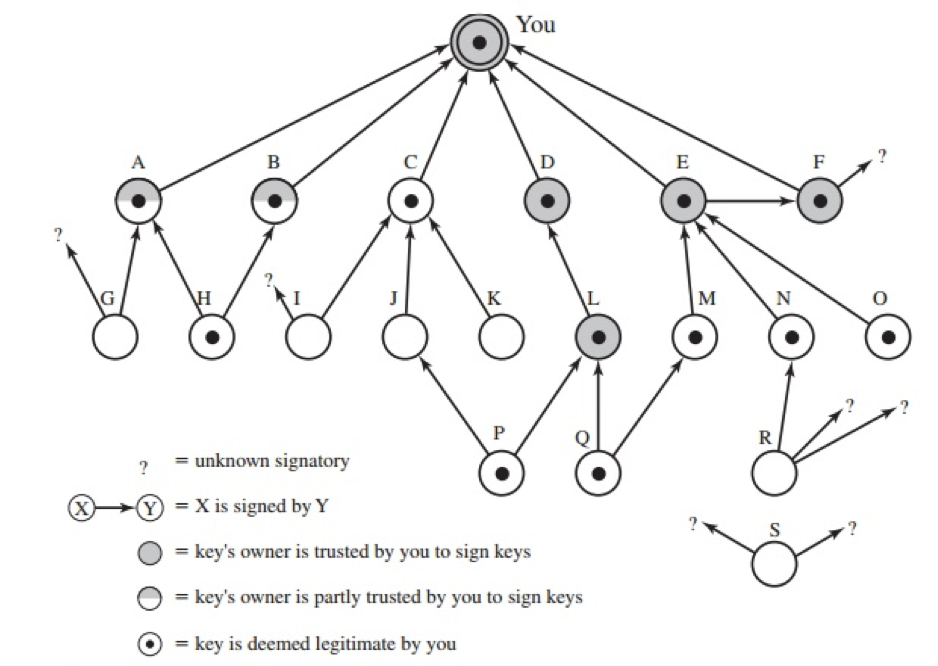
\includegraphics[width=0.7\linewidth]{Images/Chapter7/pgp-web-of-trust}
	\caption{Web of trust}
	\label{fig:pgp-web-of-trust}
\end{figure}


\section{TOR}

Figure out a way to set up internet communications so that an adversary snooping on the en route packet traffic would not be able to analyze the packet headers for the purpose of finding out who was talking to whom. Gleaning information regarding the original source of the packets and their ultimate destination is referred to as the traffic analysis attack even when protocols based on IPSec, TLS or VPN are used for establishing encrypted communication channels for the transfer of information between the web browsers and the web servers, the packet headers are always in clear text. Tor is a significant attempt to address the privacy problem over the Internet.

\subsection{Onion routing}
At each hop, the node "unwraps" a layer from the packet via symmetric keys, revealing the next destination. Clever combination of RSA and Diffie-Hellman (including its Elliptic Curve variant) cryptographic techniques.

The source of the data sends the onion to Router A, which removes a layer of encryption to learn only where to send it next and where it came from (though it does not know if the sender is the origin or just another node). Router A sends it to Router B, which decrypts another layer to learn its next destination. Router B sends it to Router C, which removes the final layer of encryption and transmits the original message to its destination \ref{fig:tor}.

\subsection{TOR basics}

Tor is based on the twin notions of Onion Proxies (OP) and Onion Routers (OR). A user’s OP first queries a Tor directory for the IP addresses of the ORs in the Tor overlay. 
An overlay network is a telecommunications network that is built on top of another network and is supported by its infrastructure. An overlay network decouples network services from the underlying infrastructure by encapsulating one packet inside of another packet.
The user then selects a subset of these ORs (typically 3) for constructing a path to the destination resource. The specification “onion” in OP and OR is related to the layers of encryption placed on the Tor messages such that, except for the user’s OP, the routing knowledge at any single node on a path through the Tor overlay is limited to exactly two nodes, the immediately preceding node on the path and the immediately following node. A user’s OP constructs a path through the Tor overlay, that is called a circuit. The two parties at the two end of a circuit may use it for an arbitrary number of TCP streams.
TCP first sets up a connection to the receiver then sends the data in segments which is carried by IP packets. This is called stream because it keeps the stream of data between to ends during transfer.


There are two types of packets: control tor packet and relay tor packets. The role of control tor packet is to alter the relationship between the sender node and the next node on the path that receives such a packet.
The role of relay tor packet is to as paths are constructed (and torn down) incrementally by a user’s OP the first link of the path can be constructed directly by the OP using a control tor packet, any extensions to the path are going to require that the commands for doing so be relayed to the currently last node on the path.

Initially, the control and the relay tor packets work together to create an end-to-end path (i.e. a circuit) in the Tor overlay in such a way that each interior node on the path has only local knowledge of the path. While the basic purpose of a relay tor packet is to carry the data that is exchanged between the two endpoints, that can only be done after a path is fully constructed. During the process of path construction, the data carried by relay tor packets is for the purpose of extending the path beyond the current termination point. Such relay tor packets generate control tor packets at the current terminal node on the path for extending the path.


\begin{figure}
	\centering
	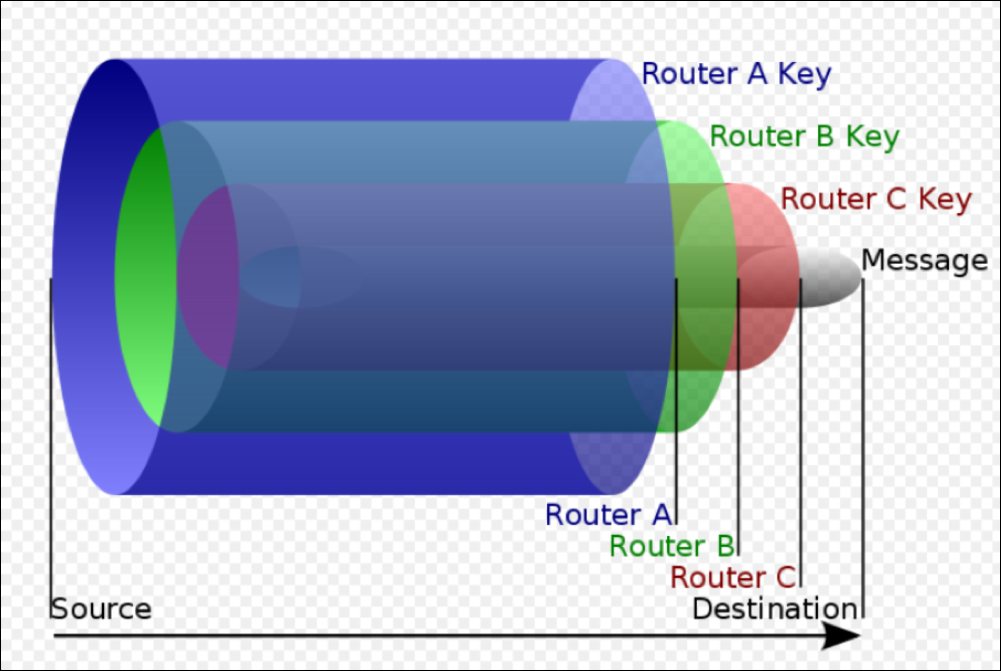
\includegraphics[width=0.7\linewidth]{Images/Chapter7/tor}
	\caption{Tor routing}
	\label{fig:tor}
\end{figure}

\subsection{Circuit creation}

How does a user’s OP use the control tor packets to create an end-to-end circuit incrementally, one hop at a time, in the Tor overlay?

We assume every OR node has a public RSA key that it makes available to the user’s OP and any communication sent to an OR that is encrypted with its RSA public key can only be understood by that OR. Next, Diffie-Hellman (DH) keys are created on the fly between the user’s OP and each of the ORs on the path chosen by the user, the purpose of the DH keys is that when the user’s OP wants to send a message to a designated OR on the path, it is encrypted with the session key derived from the OP’s DH key and that OR’s DH key. AES is used for the symmetric-key encryption with DH session keys.

The user OP (A) sends a create control tor packet to the first node (B) in the path chosen by the user. The packet contains: the CircID field (circuit identifier) set to a fresh value, the DATA field of this packet contains A's DH key Y(A$\rightarrow$B) that is encrypted with B RSA public key.
B responds back to A with the created control tor packet, B$\rightarrow$A control tor packet. The packet contains in the DATA field B's DH Y(B$\rightarrow$A). At this point, both A and B can calculate the secret session key K(AB) for their link.

All communications between any pair of nodes in the underlying network are over TLS: the public DH keys are not be visible to a packet sniffer, the RSA public/private keys used in the transmission of the control and relay tor packets are not to be confused with the RSA public/private keys used by TLS.

A and B can start exchanging relay tor packets that use the circuit identifier provided by A.  To extend the circuit, A sends B a relay tor packet with the relay extend command. The packet contains in the DATA field a DH key Y(A$\rightarrow$C) that is meant specifically for the new terminal node C on the path and also includes the identity of the new node. To guarantee that the key Y(A$\rightarrow$C) is not seen by B, it is encrypted with C's RSA public key. The DATA field in the relay extend tor packet from A to B is encrypted with the session key K(AB). When B receives the relay extend tor packet from A, it knows that it is the current endpoint on the path and generates a control tor packet for C.  B$\rightarrow$C: control tor packet, the packet contains a DATA field with A DH key Y(A$\rightarrow$C) that is meant specifically for node C and that is encrypted with C's RSA public key. This DATA field is encrypted with C RSA public key.

The control packet sent by B to C uses a new randomly generated number for the circID field that becomes the identifier for the segment of the circuit between the nodes B and C. There is no need for A to know this identifier. Only node B knows both circID identifiers (the one for the circuit between A and B and the one for the circuit between B and C). This fact plays an important role in ensuring that each node on the path has only the local knowledge of the path.
Node C responds back to B with a created control tor packet. C$\rightarrow$B: control tor packet. This packet contains a DATA field with C's DH key Y(C$\rightarrow$A) meant for A. Node B sends this acknowledgment back to A using the relay extended tor packet. B$\rightarrow$A: relay extended tor packet. This packet contains a DATA field with the key Y(C$\rightarrow$A). Now both A and C can calculate the secret session key K(AC) for any messages that A may want to send to C through B that B is not allowed to see.

The path may be extended in the same manner to the node D by using a combination of control and relay tor packets. Notice that, in constructing the end-to-end circuit, there was never a need for using A's public RSA key. As a consequence, the user A remains anonymous to all the ORs in the circuit. But all the ORs in a circuit are known to the user A. This is somehow obvious since, remember, A has chosen all the nodes in the circuit \ref{fig:tor1}.

\begin{figure}
	\centering
	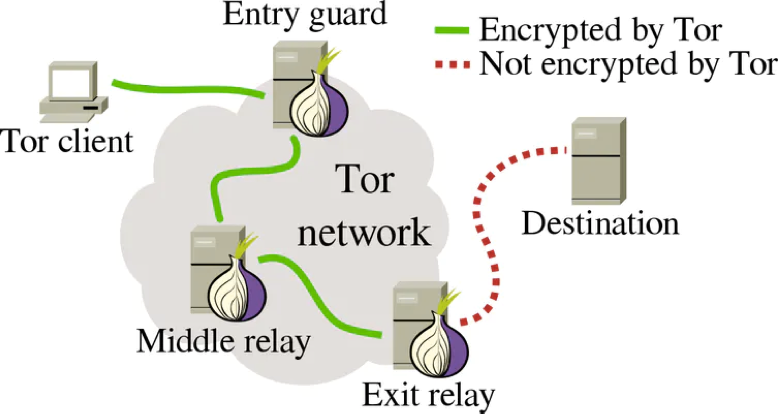
\includegraphics[width=0.7\linewidth]{Images/Chapter7/tor1}
	\caption{The circuit}
	\label{fig:tor1}
\end{figure}
To sum up:
\begin{itemize}
	\item [1.] The user OP A gets the public keys of the OR
	\item [2.] The user OP A sends a control tor packet to node B. This control is encrypted with B RSA public key. This control tor packet contains the CircID and the DH public key (A$\rightarrow$B)
	\item [3.] B Receives this and sends back its DH public key (B$\rightarrow$A). At this point A and B know K(AB) and can communicate and encrypt their communication using AES
	\item [4.] To extends the circuit, user OP A sends an extend control packet to B that is encrypted with K(AB) and contains the public DH key (A$\rightarrow$C), and is encrypted with C RSA public key.
	\item [5.] B Receives this packet and creates a control tor packet from B to C with a brand new CircID. This packet contains the public DH key (A$\rightarrow$C) encrypted with C RSA public key.
	\item [6.] C receives this packet and answers with DH public key (C$\rightarrow$A), that is sent to B and then forwarded  to A. At this point A and C can start communicating with K(AC), and use it for any message that A don't want to be seen to B.
	\item [7.] The path can be extended by repeating steps 4..6
	
	
	
\end{itemize}
\subsection{Using the circuit}


A can start pushing data into the circuit that is meant for the final destination E. Preliminarily, A sends a relay begin tor packet to B, from where it is forwarded to the next node on the circuit, and so on, thus creating an end-to-end stream between A and E. The user A is allowed to create an arbitrary number of streams sharing the same circuit. While the different TCP streams will have different streamID values in the relay
tor packets that carry the stream data, they will have the same value for the circID field. Even though the value of this circID field will change from hop to hop in a circuit.

Assume the following path in the Tor overlay: A $\rightarrow$ B $\rightarrow$ C $\rightarrow$ D. The stream data that the user A places on the wire is encrypted with the K(AD) session key, followed by its encryption with K(AC) session key, followed by its encryption by K(AB) session key. As these stream data bearing relay data tor packets are received by B from A, the node B uses the session key K(AB) to decrypt the top layer of encryption and forward the stream to node C in the circuit. This process continues until the stream data reaches the final node D, from where it goes via the normal TCP transmission to the application running at the destination E.

Can the exit node operator see the source IP address, meaning the IP address of node A? In principle, the answer is no, i.e. it should not be possible for the exit node to know the source IP address. This is so because the Tor logic that keeps A’s IP address shielded from the exit node D is the same as the logic that keeps B’s IP address shielded from D. The packets that go out from D to the web server at E should only bear D’s IP address in the source fields. When D receives replies to those packets from the web server, it simply forwards them back to C. Unfortunately, there is an attack that allows the exit node operator to identify the IP address of the source.

Can the exit node operator see the data payload of the source packet? If node A is trying to reach an HTTPS web site, that implies the usage of encryption of the payload in the packets. In that case, the exit node operator obviously cannot see inside the packets that A is sending out.